% !TEX root = Master.tex

The procedure is continued also for key category cluster 8 with the same conditions, since we have similar initial situations as in the previous two clusters.
\\

Maximum likelihood estimation return parameters $\hat{\mu} = 7.21$, $\hat{\sigma} = 0.27$ and $\hat{\nu} = 0.46$ of the log-sales of \ac{KCC} 8 fitted to an ex-Gaussian distribution with no regressors.
\autoref{fig:kcc_8_margin} summarizes the findings in a histogram of the log-sales along with an ex-Gaussian density curve with respect to the estimated parameters (\autoref{fig:kcc_8_density}) as well as the corresponding QQ-plot, where the points approximate the diagonal line (\autoref{fig:kcc_8_qqplot}). Normality of the residuals can be assumed, as the Shapiro-Wilk test returns a p-value of 0.99 and thus fails to reject the null hypothesis of normality. A histogram of the residuals and their density curve are shown in \autoref{fig:res_kcc_8_no_covariates}.\\
 Despite the high p-value of the Shapiro-Wilk test, flexible estimation of the parameters including explanatory variables should be able to provide a better overall fit to the aggregated demand quantities of this cluster. Subsequently, we enter the \ac{GAMLSS} framework to obtain time-varying parameters and therefore enhance the estimation procedure.
\\


%
%\begin{table}[H]
%\setlength\arrayrulewidth{1pt}  
%\centering
%\begin{adjustbox}{max width=\textwidth}\
%\begin{tabular}{|c|c|c|}
%\hline
%\rowcolor{lightgray} 
%$\hat{\mu}$ & $\hat{\sigma}$ & $\hat{\nu}$ \\ \hline
%7.21        & 0.27           & 0.46        \\ \hline
%\end{tabular}
%\end{adjustbox}
%\caption{Estimated parameters for log-sales of KCC 8 fitted to ex-Gaussian distribution with no covariate effects}
%\label{tab:estimated_parameters_kcc_8_no_covariates}
%\end{table}



 \begin{figure}[H]
\centering
\begin{subfigure}{.45\textwidth}
  \centering
  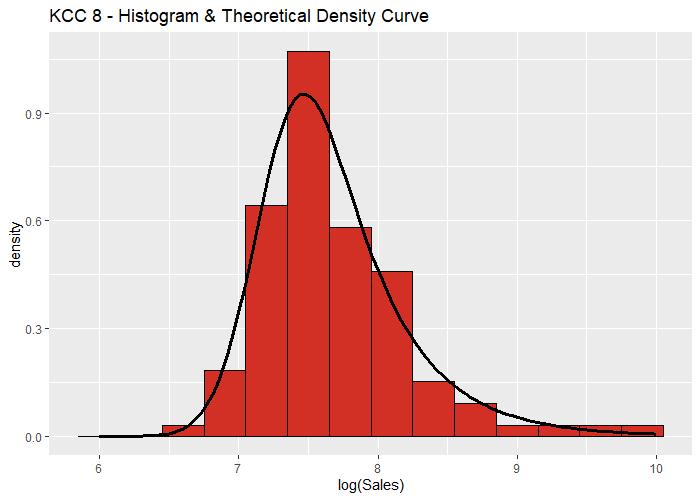
\includegraphics[width=\linewidth]{figures/kcc_8_density.png}
  \caption{Histogram \& theoretical density}
  \label{fig:kcc_8_density}
\end{subfigure}
\begin{subfigure}{.45\textwidth}
  \centering
  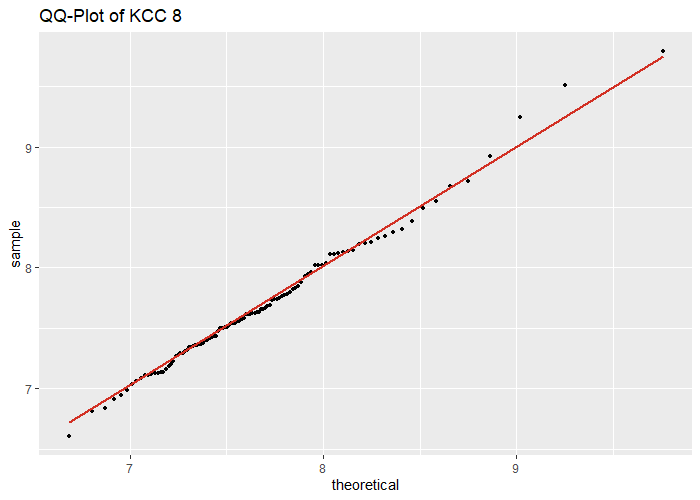
\includegraphics[width=\linewidth]{figures/kcc_8_qqplot.png}
  \caption{QQ-plot}
  \label{fig:kcc_8_qqplot}
\end{subfigure}
\caption{ex-Gaussian distribution fitted to log-sales of \ac{KCC} 8}
\label{fig:kcc_8_margin}
\end{figure} 


\begin{figure}[H]
\centering
  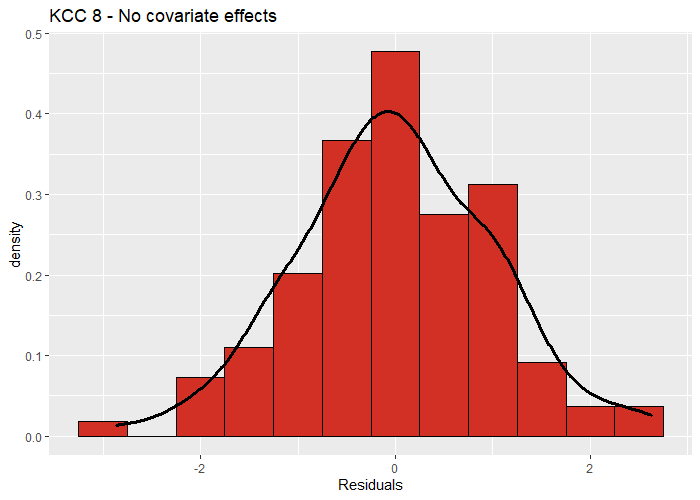
\includegraphics[width=0.45\linewidth]{figures/res_kcc_8_no_covariates.png}
  \caption{Residuals of KCC 8 log-sales fitted to an ex-Gaussian distribution with no covariate effects together with their density curve}
  \label{fig:res_kcc_8_no_covariates}
\end{figure}




Again, Model \ref{eq:gamlss_kcc_2} (see Subsection \ref{sssec:kcc_26}) is applied to the logarithmized values of the demand quantities. The estimated parameters with confidence intervals are depicted in \autoref{fig:gamlss_kcc_8_estimated_parameters} ($\hat{\mu}$ and $\hat{\sigma}$) and in \autoref{tab:nu_ci_kcc_8} (skewness parameter $\hat{\nu}$). We notice that the model fit is acceptable, matching the elevated sales during promo weeks. Especially for the two Black Friday weeks, the fitted values are close to the observed values. Furthermore, the variability is strictly decreasing over time. The overall range of the standard deviation is between 0.1 and 0.3. Skewness still remains low in the data, as can be seen in \autoref{tab:nu_ci_kcc_8}.
\\



\begin{table}[H]
\setlength\arrayrulewidth{1pt}  
\centering
\begin{adjustbox}{max width=\textwidth}\
\begin{tabular}{c|c|c}
\hline
\rowcolor{white} 
\textbf{Lower} & $\hat{\nu}$ & \textbf{Upper} \\ \hline\hline
0.181        & 0.158           & 0.203        \\ \hline
\end{tabular}
\end{adjustbox}
\caption{Estimated skewness parameter $\hat{\nu}$ of GAMLSS fit with 95\% confidence interval bounds - KCC 8}
\label{tab:nu_ci_kcc_8}
\end{table}

%\VerbatimInput[frame = single, label = "GAMLSS Fit on KCC 8" ]{gamlss_fit_kcc_8_try1.txt}








\begin{figure}[H]
\centering
  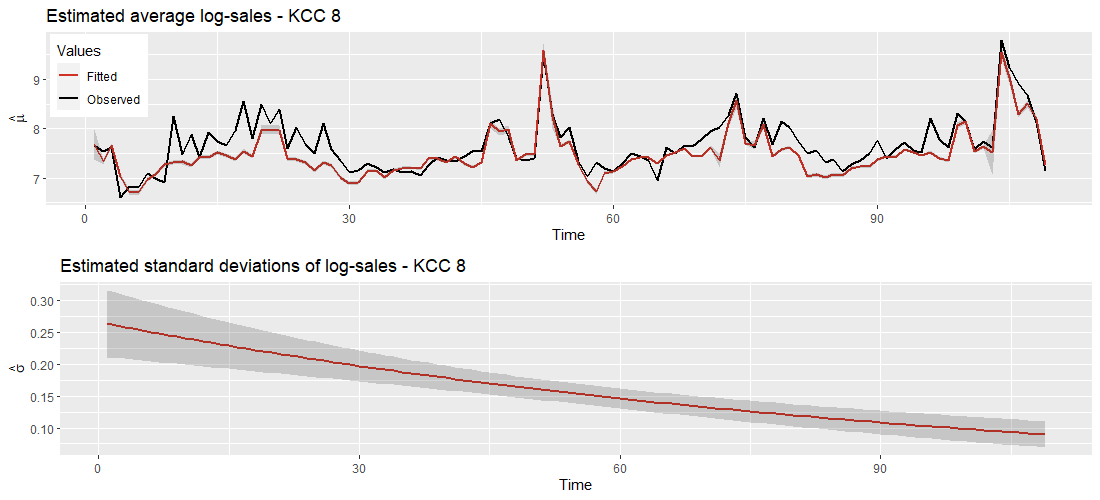
\includegraphics[width=0.95\linewidth]{figures/gamlss_kcc_8_estimated_parameters.png}
  \caption{Estimated location parameter $\hat{\mu}$ compared to the observed values and scale parameter $\hat{\sigma}$ with confidence bands of GAMLSS fit - KCC 8}
  \label{fig:gamlss_kcc_8_estimated_parameters}
\end{figure}


\autoref{fig:gamlss_effects_kcc_8} displays the effects of the covariates on the expected log-sales.
Time as well as the total markdown percentage exhibit similar positive effects on the response as in \ac{KCC} 6, collapsing into a straight line. The promotion effects seem to be more balanced, with different interquartile ranges for all three cases; Black Friday having the highest spread and Friends \& Family the highest effects in general. This pattern of boxplots for the two big promotions is therefore noticeable in the \ac{GAMLSS} fits of all three key category clusters. 
\\


\begin{figure}[H]
\centering
  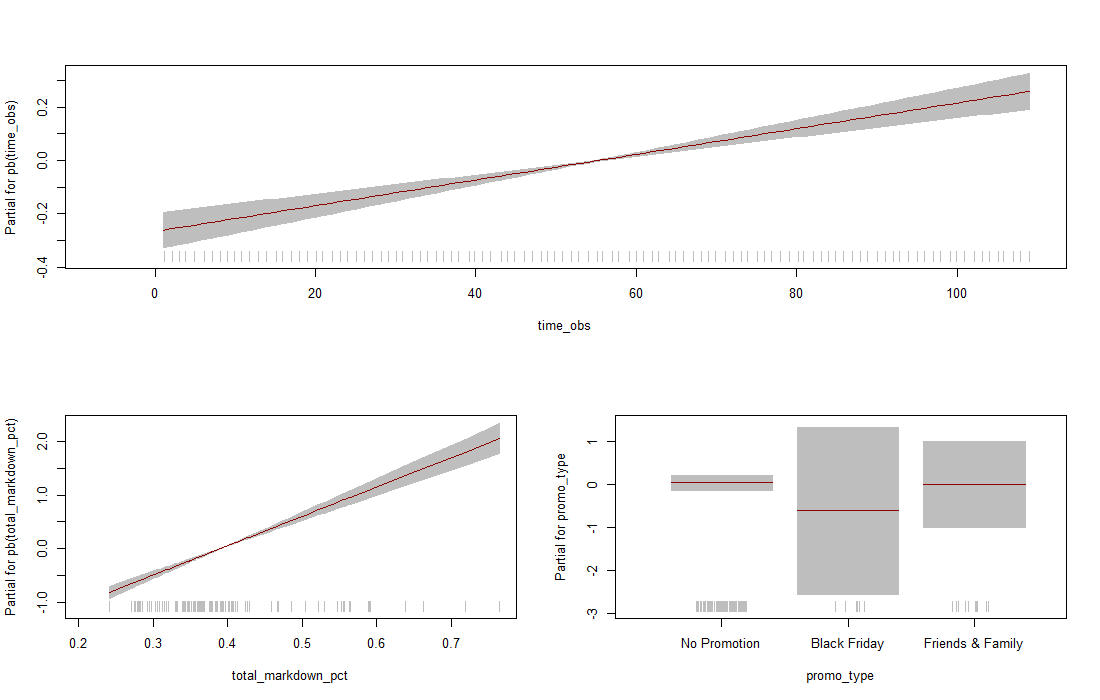
\includegraphics[width=0.95\linewidth]{figures/gamlss_effects_kcc_8.png}
  \caption{Covariate effects on the expected response variable (log-sales) of GAMLSS fit - KCC 8}
  \label{fig:gamlss_effects_kcc_8}
\end{figure}


The $\hat{\mu}$ coefficients along with standard errors and p-values are printed in \autoref{tab:gamlss_coeff_kcc_8}. The interaction between Black Friday and total markdown percentage is positive, however the standard error is relatively high resulting in a non-significant estimate. The linear effect of Black Friday is slightly negative. The interaction between markdowns and Friends \& Family is also negative, although non-significant. More details are in the \nameref{sec:appendix}, where the entire output of the model fit can be found (R output \ref{output:gamlss_fit_kcc_8_try1}).
\\


\begin{table}[H]
\centering
\begin{tabular}{l|c|c|c|l}
  \hline
  \rowcolor{white}
 \textbf{$\hat{\mu}$ Coefficients} & \textbf{Estimate} & \textbf{Std. Error} & \textbf{t value} & \textbf{p-value} \\ 
  \hline\hline
\textit{$\beta_{01}$ (Intercept)} & 5.51 & 0.17 & 31.56 & 0.00 *** \\ 
  \textit{$f_{11}$(time)} & 0.00 & 0.00 & 5.06 & 0.00 *** \\ 
  \textit{$f_{12}$(total\_markdown\_pct)} & 4.53 & 0.45 & 10.02 & 0.00 *** \\ 
  \textit{promo\_typeBlack Friday} & -0.65 & 0.37 & -1.75 & 0.08 . \\ 
  \textit{promo\_typeFriends \& Family} & -0.04 & 0.66 & -0.55 & 0.96 \\ 
  \textit{promo\_typeBlack Friday:total\_markdown\_pct} & 0.88 & 0.73 & 1.20 & 0.23  \\ 
  \textit{promo\_typeFriends \& Family:total\_markdown\_pct} & -0.76 & 1.24 & -0.62 & 0.54  \\ \hline
\end{tabular}
\caption{Estimated coefficients of \ac{GAMLSS} fit on log-sales of \ac{KCC} 8}
\label{tab:gamlss_coeff_kcc_8}
\end{table}




\begin{figure}[H]
\centering
  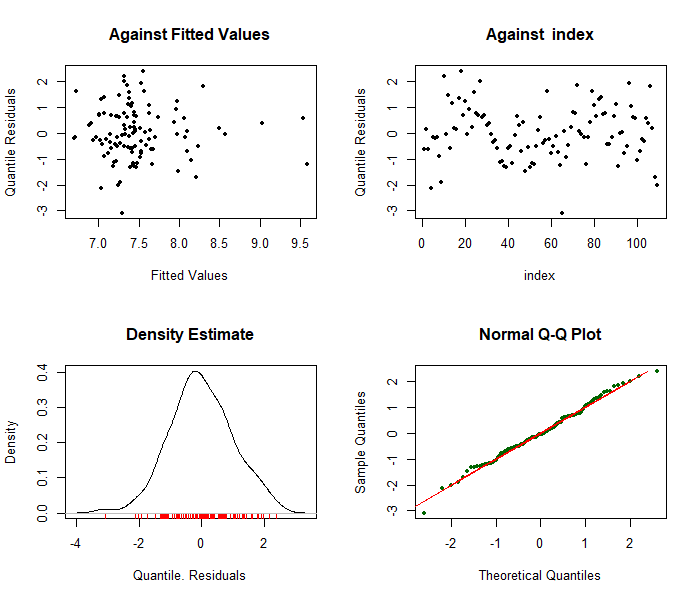
\includegraphics[width=0.95\linewidth]{figures/gamlss_residuals_kcc_8.png}
  \caption{Residuals of GAMLSS fit - KCC 8}
  \label{fig:gamlss_residuals_kcc_8}
\end{figure}






Looking at \autoref{fig:gamlss_residuals_kcc_8} and \autoref{tab:gamlss_residuals_kcc_8} for the distribution of the quantile residuals, the fitting method for this cluster is also justified. The values in \autoref{tab:gamlss_residuals_kcc_8} are close enough to those of a standard normal distribution. The diagnostic plots in \autoref{fig:gamlss_residuals_kcc_8} are in favour of a normal distribution as well, especially when looking at the QQ-plot. The Shapiro-Wilk test is "weaker" in comparison to the fit without covariate effects with a p-value of 0.86, which is still a solid reason to retain the null hypothesis of normality.
\\




%\VerbatimInput[frame = single, label = "Residuals of GAMLSS Fit on KCC 8" ]{gamlss_residuals_kcc_8.txt}


\begin{table}[H]
\centering
\begin{tabular}{c}
\hline
\rowcolor{white} 
\textbf{Summary of the Quantile Residuals} \\ \hline\hline
 $\begin{array}[t]{ r @{{}={}} l }
\text{mean} & 0.0004673878                          \\ 
\text{variance} & 1.008849                          \\ 
\text{coef. of skewness} & -0.02817569              \\ 
\text{coef. of kurtosis} & 3.04467                 \\ \hline
\end{array}$
\end{tabular}
\caption{Residuals of GAMLSS Fit on KCC 8}
\label{tab:gamlss_residuals_kcc_8}
\end{table}



%\inputRoutput[caption={Residuals of GAMLSS Fit on KCC 8},numbers=left,numberstyle=\tiny, label=output:gamlss_residuals_kcc_8]{gamlss_residuals_kcc_8.txt}


